\documentclass{article}
\usepackage{tikz}
\usetikzlibrary{arrows.meta,positioning,calc,shapes.geometric}
\pagestyle{empty}
\begin{document}
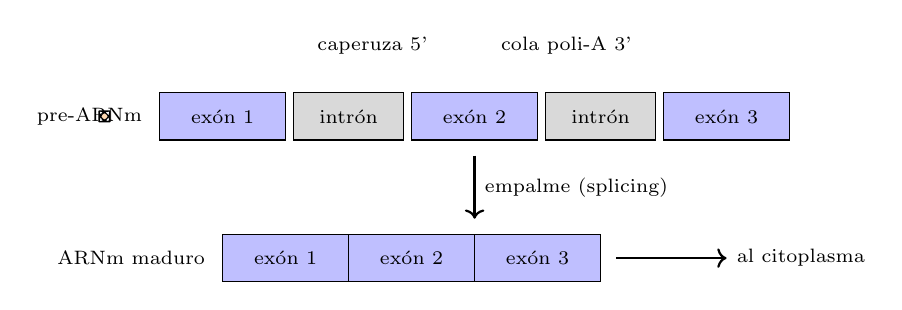
\begin{tikzpicture}

\foreach \x/\w/\c/\t in {0/1.6/blue!25/exón 1, 1.7/1.4/gray!30/intrón, 3.2/1.6/blue!25/exón 2, 4.9/1.4/gray!30/intrón, 6.4/1.6/blue!25/exón 3} {\draw[fill=\c] (\x,2.2) rectangle (\x+\w,2.8); \node[font=\scriptsize] at (\x+\w/2,2.5) {\t};}
\node[font=\scriptsize, left] at (-0.1,2.5) {pre-ARNm};
\node[draw, rounded corners, fill=orange!30, font=\scriptsize, inner sep=2pt] at (-0.7,2.5) {};
\node[font=\scriptsize] at (4,3.4) {caperuza 5' \quad \quad \quad cola poli-A 3'};
\draw[->, thick] (4,2.0) -- (4,1.2) node[midway, right, font=\scriptsize] {empalme (splicing)};
\foreach \x/\w/\t in {0.8/1.6/exón 1, 2.4/1.6/exón 2, 4.0/1.6/exón 3} {\draw[fill=blue!25] (\x,0.4) rectangle (\x+\w,1.0); \node[font=\scriptsize] at (\x+\w/2,0.7) {\t};}
\node[font=\scriptsize, left] at (0.7,0.7) {ARNm maduro};
\draw[->, thick] (5.8,0.7) -- (7.2,0.7) node[right, font=\scriptsize] {al citoplasma};

\end{tikzpicture}
\end{document}
